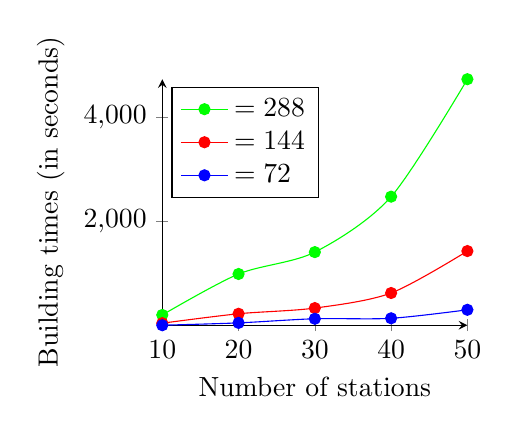
\begin{tikzpicture}
\begin{axis}[
width=.45\linewidth,
xlabel=Number of stations,
ylabel=Building times (in seconds),
legend pos=north west,
legend cell align=left,
axis x line=bottom,
axis y line=left,
]

\addplot[smooth,mark=*,color=green] plot coordinates {
(10,211)
(20,997)
(30,1417)
(40,2481)
(50,4735)
};
\addlegendentry{$\nbTimeSteps = 288$}

\addplot[smooth,mark=*,color=red] plot coordinates {
(10,53)
(20,234)
(30,343)
(40,632)
(50,1437)
};
\addlegendentry{$\nbTimeSteps = 144$}

\addplot[smooth,mark=*,color=blue] plot coordinates {
(10,14)
(20,59)
(30,138)
(40,147)
(50,310)
};
\addlegendentry{$\nbTimeSteps = 72$}

\end{axis}
\end{tikzpicture}